
\chapter{Inference for categorical data}
\label{inferenceForCategoricalData}

Statistical inference is concerned primarily with understanding the
accuracy of parameter estimates. While the equations and details change
depending on the setting, the foundations for inference are the same
throughout all of statistics. We introduce these common themes in
Sections~\ref{pointEstimates}-\ref{hypothesisTesting} by discussing
inference about the population proportion, $p$.
In Sections~\ref{}-\ref{}, we'll expand
to the application of comparing two proportions against each other.
Finally, we'll complete this chapter by analyzing categorical data
where there are many levels.

Each of the ideas in this chapter are applicable to a broad set of
applications and new contexts. We'll expand on these ideas in later
chapters.

\Comment{Do additional checks to confirm that the term
\emph{standard error} is being used consistently rather than
\emph{standard deviation}.}


%__________________
\section[Point estimates and sampling variability]{Point
    estimates and sampling variability} %\sectionvideohref{youtube-DNIauUrRIEM&list=PLkIselvEzpM7Pjo94m1e7J5jkIZkbQAl4}~\sectionslideshref{gdoc_os3_slides_4-1}}
\label{pointEstimates}

\index{data!solar survey|(}

\newcommand{\pewsolarpollsize}{1000}
\newcommand{\pewsolarpollprop}{0.887}
\newcommand{\pewsolarpollpropcomplement}{0.113}
\newcommand{\pewsolarpollpercent}{88.7}
\newcommand{\pewsolarpollpercentcomplement}{11.3}
\newcommand{\pewsolarpollcount}{887}
\newcommand{\pewsolarpollcountcomplement}{113}
\newcommand{\pewsolarpollse}{0.0100}

Pew Research conducted a poll in 2018 gauging public opinion of
American adults on solar and wind energy. They surveyed 1,000
Americans and found that \pewsolarpollpercent{}\% of respondents
favored expanding
solar energy.\footnote{The full survey's sample size was 2541,
and we've taken a subsample. To find the survey details, see\\
\oiRedirect{textbook-pew_2018_poll_on_solar_and_wind_expansion}{http://www.pewinternet.org/2018/05/14/majorities-see-government-efforts-to-protect-the-environment-as-insufficient}}
\Comment{The redirect link in the footnote needs to be confirmed as
working.}
One of the most common questions people ask about polls is
\begin{quote}
If the poll was based on only a couple thousand people, how reliable is it?
\end{quote}
If we took another poll, we wouldn't get the exact same answer.
Ultimately, it's unlikely that the actual proportion of Americans
who support expanding solar energy is \emph{exactly}
\pewsolarpollpercent{}\%, but it's probably something close to
\pewsolarpollpercent{}\%.

In this section, we discuss what a point estimate like
\pewsolarpollpercent{}\% represents
and the uncertainty associated with such an estimate. We'll also
be using some new notation and terminology:
\begin{itemize}
\item The population proportion will be written as $p$, which
    is called a \term{parameter} of the population. In the solar
    survey, $p$ represents the proportion of \emph{all}
    American adults who support solar energy. It's rare
    that we know the parameter. Instead, we often
    take a sample and compute an estimate.
\item Using Pew Research sample, we can estimate that the proportion
    of American adults who support expanding solar energy is
    \pewsolarpollpercent{}\%.
    This is called the \term{sample proportion}, and it gets a special
    label of $\hat{p}$ (spoken as \emph{p-hat}).
\item The \termsub{size of a sample}{sample size} will generally
    be denoted by $n$. In the case of this Pew Research poll,
    $n = \pewsolarpollsize{}$.
\end{itemize}

\subsection{Point Estimates}

\index{point estimate|(}

The sample proportion $\hat{p} = \pewsolarpollprop{}$ is called
the \term{point estimate} of the parameter $p$, since based
on the sample, this is our single best estimate of $p$.

The poll provides a \term{point estimate} of the actual proportion
of American adults that support expanding solar energy.
This estimate of \pewsolarpollpercent{}\% is unlikely to be perfect,
and it's quite possible for the \term{true proportion}
(a.k.a. the population proportion) to be a little lower
or a little higher. The difference between a point estimate
and the parameter is called the estimate's \term{error}.

\Comment{Should we aggressively cut out the usage of ``true''
  in the way it is used above?}

The error varies from one sample to the next: maybe
in one sample it is 1\% too low while in another
it is 3\% too high. Unfortunately, we rarely know the direction
or size of the error in our estimates, so instead we focus
on understanding what kinds of errors are typical.


\subsection{Understanding the variability of a point estimate}
\label{simulationForUnderstandingVariabilitySection}

We want to understand \emph{how does the
sample proportion $\hat{p}$ behave when the population
proportion is about \pewsolarpollprop{}}. We could
run the survey again to see how consistent the results
are, but who has the time and money for that? Instead,
we can investigate the properties of $\hat{p}$ using simulations.

To simulate the sample, we'll suppose that the population
proportion is exactly \pewsolarpollpercent{}\%.
%Now, we know
%the population proportion isn't exactly \pewsolarpollpercent\%,
%but we do expect it to be close, so this simulation will offer
%us some insights about the property of $\hat{p}$.
%If we took a random sample
%from this population, how accurate would the point estimate be?
Here's how we might simulate it:
\begin{enumerate}
\item There were about 250 million American adults in 2018.
    On 250 million pieces of paper, write ``support''
    on \pewsolarpollpercent{}\% of them and ``not'' on
    the other \pewsolarpollpercentcomplement{}\%.
\item Mix up the pieces of paper and pull out \pewsolarpollsize{}
    pieces to represent our sample of 1000 American adults.
\item Compute the fraction of the sample that say ``support''.
\end{enumerate}
Any volunteers to conduct this simulation? Probably not. Running
this simulation with 250 million pieces of paper would be
time-consuming and very costly, but we can simulate it
using computer code; we've written a short program in the
footnote.\footnote{Code using the statistical software called \R: \\
\texttt{\# 1. Create a set of 250 million entries,
where 89\% of them are "support" and 11\% are "not". \\
possible\_entries <- rep(c("support", "not"),
    c(\pewsolarpollprop{}, \pewsolarpollpropcomplement{}) * 250e6)\\
\# 2. Sample \pewsolarpollsize{} of the entries. \\
sampled\_entries <- sample(possible\_entries, \pewsolarpollsize{}) \\
\# 3. Count the number that are "justified", then divide
by the sample size. \\
sum(sampled\_entries == "justified") / \pewsolarpollsize{}}}
In this simulation, the sample gave a point estimate of
$\hat{p}_1 = 0.901$. We~know the population proportion
in this simulation is $p = \pewsolarpollprop{}$, so we know
the estimate had an error of +0.014.

One simulation isn't enough to get a sense of the null
distribution, so we should run more simulations. In a second
simulation, we get $\hat{p}_2 = 0.892$, which has an error of
+0.005.
In another, $\hat{p}_3 = 0.885$ for an error of -0.002. And in another,
an estimate of $\hat{p}_4 = 0.866$ with an error of -0.021.
With the help of a computer, we've run the simulation 10,000 times
and created a histogram of the results from all 10,000 simulations
in Figure~\ref{sampling_10k_prop_887p}. This
distribution of sample proportions is called a
\term{sampling distribution}.
%\footnote{Here is the code for 10,000 simulations: \\
%\texttt{people <- rep(c("justified", "not"), c(0.56, 0.44) * 247e6) \\
%sim.results <- c() \\
%for (i in 1:10000) \{ \\
%\ \hspace{5mm}sampled.people <- sample(people, 1000) \\
%\ \hspace{5mm}sim.results[i] <- mean(sampled.people == "justified") \\
%\} \\
%hist(sim.results, 20)} \\
%(There's actually a more efficient way to write this code, but we have provided you the long version!)}
We can characterize this sampling distribution as follows:
\begin{description}
\item[Center.] The center of the distribution is
    $\bar{x}_{\hat{p}} = \pewsolarpollprop{}0$, which is the same as the
    population proportion.
    That~is, we see that the sample proportion is an
    \term{unbiased estimate} of the population proportion.
\item[Spread.] The standard deviation of the distribution
    is $s_{\hat{p}} = \pewsolarpollse{}$. When we're talking about
    a sampling distribution or the variability of
    a point estimate, we typically use the term
    \termsub{standard error}{standard error (SE)}
    rather than \emph{standard deviation},
    and the notation $SE_{\hat{p}}$ is used for the standard
    error associated with the sample proportion.
\item[Shape.] The distribution is symmetric and bell-shaped,
    and it \emph{resembles a normal distribution}.
\end{description}
These findings are very encouraging! When the population
proportion is $p = \pewsolarpollprop{}$ and the sample size is
$n = \pewsolarpollsize{}$,
the sample proportion $\hat{p}$ tends to give a pretty good estimate
of the population proportion. We also have this interesting observation
that the histogram resembles a normal distribution.

\begin{figure}
   \centering
   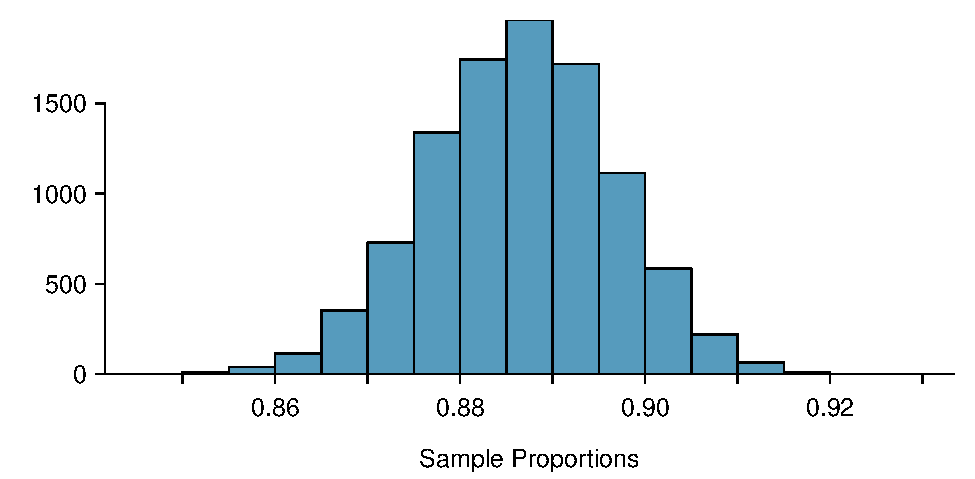
\includegraphics[width=0.8\textwidth]{ch_inference_for_props/figures/sampling_10k_prop_887p/sampling_10k_prop_887p}
   \caption{A histogram of 10,000 sample proportions, where each
       sample is taken from a population where the population of
       proportion is \pewsolarpollprop{} and the sample size is
       $n = \pewsolarpollsize{}$.}
   \label{sampling_10k_prop_887p}
\end{figure}

\begin{tipBox}{\tBoxTitle{Sampling distributions are something we
    keep in mind, even if they are never observed}
  In real-world applications, we never actually observe the
  sampling distribution, yet it is useful to always think of
  the sample proportion as coming from such a distribution.
  Understanding the distribution will help us characterize
  and make sense of the individual point estimate that we
  do observe.}
\end{tipBox}

\begin{example}{If we used a much smaller sample size of $n = 50$,
would you guess that the standard error for $\hat{p}$ would be larger
or smaller than when we used $n = \pewsolarpollsize{}$?}
\label{smallerSampleWhatHappensToPropErrorExercise}
Intuitively, it seems like more data is better
than less data, and generally that is correct! The typical error
when $p = \pewsolarpollprop{}$ and $n = 50$ would be larger
than the error we would expect when $n = \pewsolarpollsize{}$.
\end{example}

%\noindent
Example~\ref{smallerSampleWhatHappensToPropErrorExercise}
highlights an important property: a bigger sample
tends to provide a more precise point estimates than a smaller sample.

\index{point estimate|)}


\subsection{Central Limit Theorem}

The distribution in
Figure~\ref{sampling_10k_prop_887p} looks an awful lot like
a normal distribution. That is no anomaly; it is the result
of a general principle called the \term{Central Limit Theorem}.
\index{Central Limit Theorem!proportion|textbf}

\begin{termBox}{\tBoxTitle{Central Limit Theorem for proportions
    \& the success-failure condition}
When the observations are independent and the sample size is
sufficiently large, the sample proportion $\hat{p}$ will tend
to follow a normal distribution with the following mean and
standard error:
\begin{align*}
  \mu_{\hat{p}} &= p
  &SE_{\hat{p}} &= \sqrt{\frac{p (1 - p)}{n}}
\end{align*}
The sample size is typically considered sufficiently large when
$np \geq 10$ and $n(1-p) \geq 10$, which is called the
\term{success-failure condition}.} %since $np$ represents the
%number of expected \emph{successes} and $n(1-p)$ the expected
%number of \emph{failures}.}
\end{termBox}

The Central Limit Theorem is incredibly important, and it provides
a foundation for the rest of this book. As we begin applying
this principle, be mindful of the two requirements:
the observations must be independent, and the the sample size must
be sufficiently large such that $np \geq 10$ and $n(1-p) \geq 10$.

\begin{example}{Earlier we estimated the mean and standard
error of the $\hat{p}$'s using simulated data when
$p = \pewsolarpollprop{}$ and $n = \pewsolarpollsize{}$.
Confirm that the distribution is approximately
normal.}\label{sample_p887_n1000_confirm_normal}
\begin{description}
\item[Independence.] There are $n = \pewsolarpollsize{}$
    observations for each
    sample proportion $\hat{p}$, and each of those observations
    are independent draws. \emph{The most common way for
    observations to be considered independent is if they are from
    a simple random sample.}
    \index{independent}
    \index{independence}
    \index{Central Limit Theorem|independence}
\item[Success-failure condition.] We can confirm the sample size
    is sufficiently large by checking the success-failure condition
    and confirming each of the following values are greater than 10:
    \begin{align*}
    np &= \pewsolarpollsize{} \times \pewsolarpollprop{}
        = \pewsolarpollcount{}
    &n(1-p) &= \pewsolarpollsize{} \times (1 - \pewsolarpollprop{})
        = \pewsolarpollcountcomplement{}
    \end{align*}
\end{description}
Both of the independence and success-failure conditions are
satisfied, so the Central Limit Theorem applies and the normal
distribution is reasonable in this context!
\end{example}

\begin{example}{Compute the theoretical mean and standard error
of the $\hat{p}$'s when
$p = \pewsolarpollprop{}$ and $n = \pewsolarpollsize{}$,
according to the
Central Limit Theorem.}\label{sample_p887_n1000_mean_se}
The mean of the $\hat{p}$'s is simply the population proportion:
$\mu_{\hat{p}} = \pewsolarpollprop{}$.

The calculation of the standard error of $\hat{p}$ uses
the following formula:
\begin{align*}
SE_{\hat{p}}
    = \sqrt{\frac{p (1 - p)}{n}}
    = \sqrt{\frac{\pewsolarpollprop{} (1 - \pewsolarpollprop{})}{1000}}
    = \pewsolarpollse{}
\end{align*}
\end{example}

\begin{example}{Estimate how frequently the sample proportion
$\hat{p}$ should be within 0.02 (2\%) of the population value,
$p = \pewsolarpollprop{}$. Based on
Examples~\ref{sample_p887_n1000_confirm_normal}
and~\ref{sample_p887_n1000_mean_se}, we know that the distribution is
$N(\mu_{\hat{p}} = \pewsolarpollprop{}, SE_{\hat{p}} = \pewsolarpollse{})$.}
\label{sampling_10k_prop_887p-prop_from_867_to_907}
After so much practice in Section~\ref{normalDist},
this example will hopefully feel familiar!
We would like to understand the fraction of $\hat{p}$'s
between 0.867 and 0.907:
\begin{center}
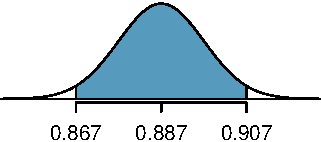
\includegraphics[width=60mm]{ch_inference_for_props/figures/p-hat_from_867_and_907/p-hat_from_867_and_907}
\end{center}
With $\mu_{\hat{p}} = \pewsolarpollprop{}$ and
$SE_{\hat{p}} = \pewsolarpollse{}$,
we can compute the Z-score for both the left and right cutoffs:
\begin{align*}
Z_{0.867} &= \frac{0.867 - \pewsolarpollprop{}}{\pewsolarpollse{}} = -2
&Z_{0.907} &= \frac{0.907 - \pewsolarpollprop{}}{\pewsolarpollse{}} = 2
\end{align*}
We can use either statistical software, a graphing calculator,
or a table to find the areas to the tails, and in any case we
will find that they are each 0.0228. The total tail areas are
$2 \times 0.0228 = 0.0456$, which leaves the shaded area of
0.9544. That is, about 95.44\% of the sampling distribution
in Figure~\ref{sampling_10k_prop_887p} is within $\pm0.02$
of the simulation population proportion, $p = \pewsolarpollprop{}$.
%of these
%cutoffs and compute the difference of these areas
%to get the central area:
%\begin{center}
%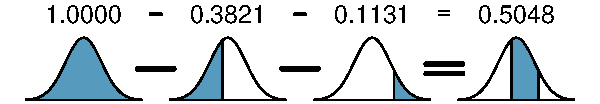
\includegraphics[width=60mm]{ch_inference_for_props/figures/p-hat_from_53_and_59_computation/p-hat_from_53_and_59_computation}
%\end{center}
\end{example}

\begin{exercise}
In Example~\ref{smallerSampleWhatHappensToPropErrorExercise}
we discussed how a smaller sample would tend
to produce a less reliable estimate. Explain how this intuition
is reflected in the formula for
$SE_{\hat{p}} = \sqrt{\frac{p (1 - p)}{n}}$.\footnote{Since the
sample size $n$ is in the denominator of the fraction (on the
bottom of the fraction), a bigger sample size means the entire
expression when calculated will tend to be smaller. That is,
a larger sample size would correspond to a smaller standard error.}
\end{exercise}

%In Example~\ref{sampling_10k_prop_56p}, we applied a general
%principle called the \term{Central Limit Theorem}
%\hiddenterm{Central Limit Theorem!proportions} when
%we used the normal distribution as an approximation.


\subsection{Applying the Central Limit Theorem to a real-world setting}

Think back to the 2018 poll where
$\hat{p} = \pewsolarpollprop{}$ of American adults favored
expanding solar energy. We might wonder: does the sample
proportion from the poll approximately follow a normal
distribution?
We check the conditions from the Central Limit Theorem:
\begin{description}
\item[Independence.] The poll is a simple random sample of
    American adults, which means that the observations are
    independent.
\item[Success-failure condition.] To check this condition,
    we need the population proportion, $p$, to check if both
    $np$ and $n(1-p)$ are greater than 10. However, we do not
    know the value of $p$; that's exactly why the pollsters
    took a sample! In cases like these, we often use $\hat{p}$
    as our next best way to check the success-failure condition:
    \begin{align*}
    n\hat{p} &= \pewsolarpollsize{} \times \pewsolarpollprop{}
        = \pewsolarpollcount{}
    &n (1 - \hat{p}) &= \pewsolarpollsize{} \times (1 - \pewsolarpollprop{})
        = \pewsolarpollcountcomplement{}
    \end{align*}
    While we cannot check the condition with $p$,
    $\hat{p}$ acts as a reasonable substitute, and we are comfortably
    above the minimums of 10.
\end{description}

This \term{substitution approximation} of using $\hat{p}$ in
place of $p$ will also be useful when computing the standard error
of the sample proportion in many situations:
\begin{align*}
SE_{\hat{p}}
    = \sqrt{\frac{p (1 - p)}{n}}
    \approx \sqrt{\frac{\hat{p} (1 - \hat{p})}{n}}
    \approx \sqrt{\frac{\pewsolarpollprop{}
        (1 - \pewsolarpollprop{})}{\pewsolarpollsize{}}}
    = \pewsolarpollse{}
\end{align*}
This substitution approximation technique is useful in many
situations.
%\footnote{There are additional methods
%for proportions that perform some correction for the substitution
%approximation. However, we leave those proportion methods for
%a future course.}




%__________________
\section[Confidence interval for a sample proportion]{Confidence
    intervals for\\a sample proportion} % \sectionvideohref{youtube-FUaXoKdCre4&list=PLkIselvEzpM7Pjo94m1e7J5jkIZkbQAl4}~\sectionslideshref{gdoc_os3_slides_4-2}}
\label{confidenceIntervals}

\index{confidence interval|(}

The sample proportion $\hat{p}$ provides a single plausible value
for the population proportion $p$. However, the sample proportion
isn't perfect and will have some \emph{standard error}
associated with it. Instead of supplying just this point estimate
of the population proportion, a next logical step would be
to provide a plausible \emph{range of values}.

\subsection{Capturing the population parameter}

A plausible range of values for the population parameter
is called a \term{confidence interval}.

Using only a point estimate is like fishing in a murky
lake with a spear, and using a confidence interval is
like fishing with a net. We can throw a spear where we
saw a fish, but we will probably miss. On the other hand,
if we toss a net in that area, we have a good chance of
catching the fish.

If we report a point estimate $\hat{p}$, we probably
will not hit the exact population proportion. On the
other hand, if we report a range of plausible values
-- a confidence interval -- we have a good shot at
capturing the parameter. 

\begin{exercise}
If we want to be very certain we capture the population
proportion in an interval, should we use a wider interval
or a smaller interval?\footnote{If we want to be more
certain we will capture the fish, we might use a
wider net. Likewise, we use a wider confidence interval
if we want to be more certain that we capture the
parameter.}
\end{exercise}

\subsection{An approximate 95\% confidence interval}

Our sample proportion $\hat{p}$ is the most plausible
value of the population proportion, so it makes sense
to build a confidence interval around this point estimate.
The \hiddenterm{standard error} provides a guide for how
large we should make the confidence interval.

The standard error represents the standard deviation
of the point estimate, and when the Central
Limit Theorem conditions are satisfied, we also know
that the point estimate closely follows a normal
distribution. In a normal distribution, about 95\% of
the data is within 2 standard deviations of the mean.
Using this principle, we can construct a confidence
interval that extends 2 standard errors from the sample
proportion to be \term{95\% confident}\index{confident|textbf}
that the interval captures the population proportion:
\begin{align*}
\text{point estimate}\ &\pm\ 2\times SE \\
\hat{p}\ &\pm\ 2\times SE_{\hat{p}}
%\label{95PercentConfidenceIntervalFormula}
\end{align*}
But what does ``95\% confident'' mean? Suppose we took
many samples and built a 95\% confidence interval from
each sample. Then about 95\% of those intervals would
contain the parameter, $p$.
Figure~\ref{95PercentConfidenceInterval} shows this
process with 25 samples from the simulation in
Section~\ref{simulationForUnderstandingVariabilitySection},
where 24 of the resulting confidence intervals contain
the simulation's population proportion of
$p = \pewsolarpollprop{}$, and one interval does not.

\begin{figure}
   \centering
   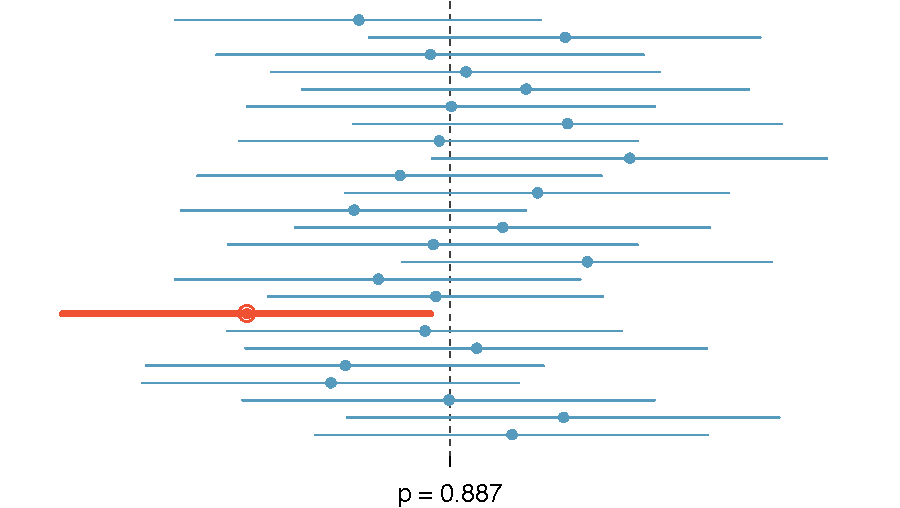
\includegraphics[width=0.75\textwidth]{ch_inference_for_props/figures/95PercentConfidenceInterval/95PercentConfidenceInterval}
   \caption{Twenty-five point estimates and confidence
       intervals from the simulations in
       Section~\ref{simulationForUnderstandingVariabilitySection}.
       For~each sample, a 95\% confidence interval was
       constructed and shown relative to the population
       proportion $p = \pewsolarpollprop{}$. Only~1 of these~25
       intervals did not capture the true population
       proportion.}
   \label{95PercentConfidenceInterval}
\end{figure}

\begin{example}{In Figure~\ref{95PercentConfidenceInterval},
one interval does not contain $p = \pewsolarpollprop{}$.
Does this imply that the population proportion cannot be
$p = \pewsolarpollprop{}$?}
Just as some observations occur more than 2 standard deviations
from the mean, some point estimates will be more than
2 standard errors from the parameter of interest.
A confidence interval only provides a plausible range
of values. While we might say other values are implausible
based on the data, this does not mean they are impossible.
\end{example}

While about 95\% of the data is within 2 standard deviations
in a normal distribution, it would be more precise to use
a value of 1.96 standard deviations. This more precise value
is typically what is used to construct confidence intervals.

\begin{termBox}{\tBoxTitle{95\% confidence interval for
    a parameter}
  When a point estimate qualifies for the Central Limit
  Theorem and closely follows a normal distribution,
  we can construct a 95\% confidence interval as
  \begin{align*}
  \text{point estimate} &\pm 1.96 \times SE
  \end{align*}}
\end{termBox}

\begin{example}{In Section~\ref{pointEstimates} we learned about
    a poll where \pewsolarpollpercent{}\% of a random sample of
    \pewsolarpollsize{} American adults
    supported expanding the role of solar power. Compute and
    interpret a 95\% confidence interval for the population
    proportion.} \label{95p_ci_for_pew_solar_support}
  We earlier confirmed that $\hat{p}$ follows a normal
  distribution and has a standard error is
  $SE_{\hat{p}} = \pewsolarpollse{}$.
  To compute the 95\% confidence interval, we plug the
  point estimate $\hat{p} = \pewsolarpollprop{}$ and
  standard error into the 95\% confidence interval formula:
  \begin{align*}
  \hat{p} \pm 1.96 \times SE_{\hat{p}}
  \quad\to\quad
  \pewsolarpollprop{} \pm 1.96 \times \pewsolarpollse{}
  \quad\to\quad
  (0.8674, 0.9066)
  \end{align*}
  We are 95\% confident that the actual proportion of
  American adults who support expanding solar power is
  between 86.74\% and 90.66\%.
\end{example}


\subsection{Changing the confidence level}
\label{changingTheConfidenceLevelSection}

\index{confidence interval!confidence level|(}

Suppose we want to consider confidence intervals where the confidence
level is somewhat higher than 95\%; perhaps we would like a confidence
level of 99\%. Think back to the analogy about trying to catch a fish:
if~we want to be more sure that we will catch the fish, we should use
a wider net. To create a 99\% confidence level, we must also widen our
95\% interval. On the other hand, if we want an interval with lower
confidence, such as 90\%, we could make our original 95\% interval
slightly slimmer.

The 95\% confidence interval structure provides guidance in how to
make intervals with new confidence levels. The general 95\% confidence
interval for a point estimate that follows the normal distribution is
normal distribution:
\begin{eqnarray}
\text{point estimate}\ \pm\ 1.96\times SE
\end{eqnarray}
There are three components to this interval: the point estimate $\hat{p}$,
``1.96'', and the standard error. The choice of $1.96\times SE$ was
based on capturing 95\% of the data since the estimate is within 1.96
standard errors of the parameter about 95\% of the time.
The choice of 1.96 corresponds to a 95\% confidence level. 

\begin{exercise} \label{leadInForMakingA99PercentCIExercise}
If $X$ is a normally distributed random variable, how often will $X$
be within 2.58 standard deviations of the mean?\footnote{This is
equivalent to asking how often the Z-score will be larger than -2.58
but less than 2.58. (For a picture, see Figure~\ref{choosingZForCI}.)
To determine this probability, we can use statistical software,
a calculator, or a table to look up -2.58 and 2.58 for the normal
distribution: 0.0049 and 0.9951. Thus, there is a
$0.9951-0.0049 \approx 0.99$ probability that an unobserved random
variable $X$ will be within 2.58 standard deviations of $\mu$.}
\end{exercise}

To create a 99\% confidence interval, change 1.96 in the 95\%
confidence interval formula to be $2.58$. Guided Practice~\ref{leadInForMakingA99PercentCIExercise} highlights
that 99\% of the time a normal random variable will be within
2.58 standard deviations of the mean. This approach -- using
the Z-scores in the normal model to compute confidence levels -- is
appropriate when $\hat{p}$ is associated with a normal distribution
with mean $p$ and standard error $SE_{\hat{p}}$. Thus, the formula
for a 99\% confidence interval for $\hat{p}$ is
\begin{eqnarray}
\hat{p}\ \pm\ 2.58\times SE_{\hat{p}}
\label{99PercCIForProp}
\end{eqnarray}

\begin{figure}
  \centering
  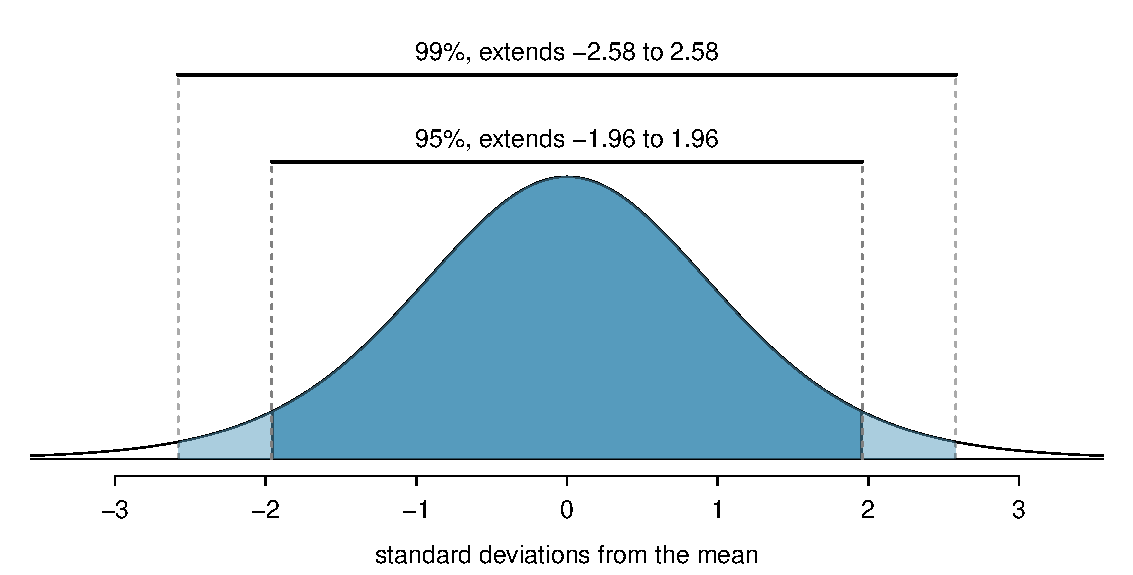
\includegraphics[width=\textwidth]{ch_inference_for_props/figures/choosingZForCI/choosingZForCI}
  \caption{The area between -$z^{\star}$ and $z^{\star}$ increases as
      $z^{\star}$ becomes larger. If the confidence level is 99\%,
      we choose $z^{\star}$ such that 99\% of the normal curve is
      between -$z^{\star}$ and $z^{\star}$, which corresponds to 0.5\%
      in the lower tail and 0.5\% in the upper tail: $z^{\star}=2.58$.}
\label{choosingZForCI}
\index{confidence interval!confidence level|)}
\end{figure}

The normal approximation is crucial to the precision of these
confidence intervals. For the context of sample proportions, the
normal distribution is reasonable to use whenever the sample
observations are independent and the success-failure condition
holds ($np$ and $n(1-p)$ are both at least 10).
For some other point estimates, the normal model is not a good fit.
In these cases, we'll use alternative distributions that better
represent the sampling distribution.

\begin{tipBox}{\tipBoxTitle[]{How to verify sample observations
    are independent}
  Subjects in an experiment are considered independent if they undergo
      random assignment to the treatment groups. \\[2mm]
  If the observations are from a simple random sample and consist
      of fewer than 10\% of the population, then they are independent.
      Even if the sample is bigger than 10\%, assuming independence
      will lead to more conservative results. \\[2mm]
  If a sample is from a seemingly random process,
      e.g. an occasional error on an assembly line,
      checking independence is more difficult. In~this case,
      use your best judgement.}
\end{tipBox}

\begin{termBox}{\tBoxTitle{Confidence interval for $p$ using any confidence level}
  If $\hat{p}$ approximately follows the normal model with
  standard error $SE_{hat{p}}$, then a confidence interval
  for the population parameter is
  \begin{eqnarray*}
  \hat{p}\ \pm\ z^{\star} SE_{\hat{p}}
  \end{eqnarray*}
  where $z^{\star}$ corresponds to the confidence level selected.}
\end{termBox}

Figure~\ref{choosingZForCI} provides a picture of how to identify
$z^{\star}$ based on a confidence level. We~select $z^{\star}$
so that the area between -$z^{\star}$ and $z^{\star}$ in the normal
model corresponds to the confidence level. 

\begin{termBox}{\tBoxTitle{Margin of error}
\label{marginOfErrorTermBox}
In a confidence interval, $z^{\star}\times SE$ is called the
\term{margin of error}.}
\end{termBox}

\begin{example}{Use the data in
    Example~\ref{95p_ci_for_pew_solar_support} to
    create a 90\% confidence interval for the proportion of American
    adults that support expanding solar power students.}
  We first find $z^{\star}$ such that 90\% of the distribution falls
  between -$z^{\star}$ and $z^{\star}$ in the standard normal model,
  $N(\mu=0, \sigma=1)$. We can do this using a graphing calculator,
  statistical software, or a probability table by looking for a lower
  tail of 5\% (the other 5\% is in the upper tail): $z^{\star}=1.65$.
  The 90\% confidence interval can then be computed as
  $\hat{p}\ \pm\ 1.65\times SE_{\hat{p}} \to (0.8705, 0.9035)$.
  (We had already verified conditions for normality and the standard error.)
  That is, we are 90\% confident that 87.1\% to 90.4\% of American
  adults support the expansion of solar power in 2018.
\end{example}



\subsection{More case studies}

\index{data!Ebola poll|(}

\newcommand{\wsjebolapollsize}{1042}
\newcommand{\wsjebolapollsizecomma}{1,042}
\newcommand{\wsjebolapollprop}{0.82}
\newcommand{\wsjebolapollpropcomplement}{0.18}
\newcommand{\wsjebolapollpercent}{82}
\newcommand{\wsjebolapollpercentcomplement}{18}
\newcommand{\wsjebolapollcount}{854}
\newcommand{\wsjebolapollcountcomplement}{188}
\newcommand{\wsjebolapollse}{0.012}


In New York City on October 23rd, 2014, a doctor who had recently been
treating Ebola patients in Guinea went to the hospital with a slight fever
and was subsequently diagnosed with Ebola. Soon thereafter,
an NBC~4 New York/The Wall Street Journal/Marist Poll found that
\wsjebolapollpercent{}\% of New Yorkers favored a ``mandatory 21-day
quarantine for anyone who has come in contact with an Ebola
patient''.\footnote{\oiRedirect{textbook-maristpoll_ebola_201410}{Poll
ID NY141026 on maristpoll.marist.edu}.} This poll included responses
of \wsjebolapollsizecomma{} New York adults between October 26th and~28th,
2014. We may want a confidence interval for the proportion of New York
adults who favored a mandatory quarantine of anyone who had been in
contact with an Ebola patient.

\begin{example}{What is the point estimate in this case,
    and is it reasonable to
    use the normal distribution to model that point estimate?}
  The point estimate, based on a sample of size $n = \wsjebolapollsize{}$,
  is $\hat{p} = \wsjebolapollprop{}$. To check whether $\hat{p}$ can be reasonably
  modeled using the normal distribution, we check independence
  (the poll is based on a simple random sample) and the
  success-failure condition
  ($\wsjebolapollsize{} \times \hat{p} \approx \wsjebolapollcount{}$
  and $\wsjebolapollsize{} \times (1 - \hat{p})
      \approx \wsjebolapollcountcomplement{}$,
  both easily greater than~10). With the conditions met, we are assured
  that the sampling distribution of $\hat{p}$ can be modeled using
  a normal distribution.
\end{example}

\begin{example}{Estimate the standard error of
    $\hat{p} = \wsjebolapollprop{}$ from the Ebola survey.}
  We'll use the substitution approximation of
  $p \approx \hat{p} = \wsjebolapollprop{}$ to compute the standard error:
  \footnote{$SE = \sqrt{\frac{p(1-p)}{n}}
    \approx \sqrt{\frac{\wsjebolapollprop{}
        (1 - \wsjebolapollprop{})}{\wsjebolapollsize{}}}
    = \wsjebolapollse{}$.}
\end{example}

\begin{example}{Construct a 95\% confidence interval for $p$,
    the proportion of New York adults who supported a quarantine
    for anyone who has come into contact with an Ebola patient.}
  Using the standard error $SE = 0.012$ from
  Example~\ref{seOfPropOfAmericansJobApprovalOfSupremeCourt},
  the point estimate \wsjebolapollprop{}, and $z^{\star} = 1.96$
  for a 95\% confidence interval, the confidence interval is
  \begin{eqnarray*}
  \text{point estimate} \ \pm\ z^{\star}SE
    \quad\to\quad \wsjebolapollprop{} \ \pm\ 1.96\times \wsjebolapollse{}
    \quad\to\quad (0.796, 0.844)
  \end{eqnarray*}
  We are 95\% confident that the proportion of New York adults
  in October 2014 who supported a quarantine for anyone who had come
  into contact with an Ebola patient was between 0.796 and 0.844.
\index{data!Ebola poll|)}
\end{example}

\begin{exercise}
Do you think the confidence interval is still valid for the opinions
of New Yorkers today?\footnote{No. The poll was taken at a
time where there was a huge public safety concern. Now that people
have had some time to step back, they may have changed their opinions.
We would need to run a new poll if we wanted to get an estimate of the
current proportion of New York adults who would support such a
quarantine period.}
\end{exercise}

\index{data!wind turbine survey|(}

\newcommand{\pewwindpollsize}{\pewsolarpollsize}
\newcommand{\pewwindpollprop}{0.848}
\newcommand{\pewwindpollpropcomplement}{0.152}
\newcommand{\pewwindpollpercent}{84.8}
\newcommand{\pewwindpollpercentcomplement}{15.2}
\newcommand{\pewwindpollcount}{848}
\newcommand{\pewwindpollcountcomplement}{152}
\newcommand{\pewwindpollse}{0.0114}

In the poll by Pew Research asking about solar energy, the
researchers also inquired about other forms of energy.
In this next case study, we examine the support for expanding wind
turbines, which received support from \pewwindpollpercent{}\%
of the \pewwindpollsize{} respondents.

\begin{exercise}\label{pew_wind_turbine_support_normal_dist_gp}
Is the normal approximation reasonable in this case?\footnote{We
check independence, which is okay since this survey was a simple
random sample, and also the success-failure condition
($\pewwindpollsize{} \times \pewwindpollprop{} = \pewwindpollcount{}$
and $\pewwindpollsize{} \times \pewwindpollpropcomplement{}
    = \pewwindpollcountcomplement$ are both at least 10).
Since both are satisfied, $\hat{p} = \pewwindpollprop{}$ can be
modeled using the normal distribution.}
\end{exercise}

\begin{exercise}
Using the Pew Research survey where $n = \pewwindpollsize{}$ and
$\hat{p} = \pewwindpollprop{}$, create a 99\% confidence interval
for the level of American support for expanding the use of wind
turbines for power
generation.\footnote{Guided
Practice~\ref{pew_wind_turbine_support_normal_dist_gp}
confirmed that that $\hat{p}$ closely follows a normal distribution,
so we can use the confidence interval formula:
\begin{align*}
\text{point estimate} \pm z^{\star} SE
\end{align*}
In this case, the point estimate is $\hat{p} = \pewwindpollprop{}$.
For a 99\% confidence interval, $z^{\star} = 2.58$. Computing the
standard error:
$SE_{\hat{p}}
  = \sqrt{\frac{\pewwindpollprop{}(1 - \pewwindpollprop{})}
      {\pewwindpollsize{}}}
  = \pewwindpollse{}$.
Finally, we compute the interval as
$\pewwindpollprop{} \pm 2.58 \times \pewwindpollse{} \to (0.8186, 0.8774)$.
It is also \emph{always} important to provide an interpretation for
the interval: we are 99\% confident the proportion of
Americans adults that support expanding the use of wind
turbines is between 81.9\% and 87.7\% in 2018.}
\end{exercise}




\subsection{Interpreting confidence intervals}
\label{interpretingCIs}

\index{confidence interval!interpretation|(}

In each of the examples, we described the confidence
intervals by putting them into the context of the data and also
using somewhat formal language:
\begin{description}
  \item[Solar.] We are 90\% confident that 87.1\% to 90.4\% of
      American adults support the expansion of solar power in 2018.
  \item[Ebola.] We are 95\% confident that the proportion
      of New York adults in October 2014 who supported a quarantine
      for anyone who had come into contact with an Ebola patient was
      between 0.796 and 0.844.
  \item[Wind Turbine.] We are 99\% confident the proportion of
      Americans adults that support expanding the use of wind
      turbines is between 81.9\% and 87.7\% in 2018.
\end{description}
First, notice that the statements are always about the population
parameter, which considers all American adults for the energy polls
and all New York adults for the quarantine poll, \emph{not} only
the adults included in the sample.

We also avoided another common mistake:
\emph{incorrect} language might try to describe the confidence interval
as capturing the population parameter with a certain probability.
Making a probability interpretation is a common error:
while it might be useful to think of it as a probability,
the confidence level only quantifies how plausible
it is that the parameter is in the interval.

Another important consideration of confidence intervals is that they
\emph{only try to capture the population parameter}. A confidence
interval says nothing about the confidence of capturing individual
observations, a proportion of the observations, or about capturing
point estimates. Confidence intervals only attempt to capture
population parameters.

\index{data!wind turbine survey|)}
\index{data!solar survey|)}
\index{confidence interval!interpretation|)}

\CalculatorVideos{confidence intervals for a single proportion}

\index{confidence interval|)}




%__________________
%\section[Hypothesis testing]{Hypothesis testing \sectionvideohref{youtube-NVbPE1_Cbx8&list=PLkIselvEzpM7Pjo94m1e7J5jkIZkbQAl4}~\sectionslideshref{gdoc_os3_slides_4-3}}
\section{Hypothesis testing for a proportion}
\label{hypothesis_testing_one_prop}
\label{hypothesisTesting}

\index{hypothesis testing|(}

Warren Buffett is a legendary investor who has made a fortune
of about \$85~billion in the stock market. His net worth is
more than the gross domestic product of dozens of countries.
As perhaps the most thoughtful investors of our time, Buffett
has advised people to steer clear of hedge funds and instead
invest directly in an index
fund.\footnote{\oiRedirect{buffett-invest-in-index-fund}{www.cnbc.com/2018/01/03/why-warren-buffett-says-index-funds-are-the-best-investment.html}}
\Comment{Make sure the URL link goes where it should.}

Buffett's suggestion is that hedge funds tend to give lower
rates of return than index funds, and it is helpful to test
that theory! We'll look at a sample of managed funds
and see whether these funds tend to beat or fall behind a
standard index fund.






%There's an adage in United States financial markets that
%it is better to get out of investments during the six ``summer''
%months: \emph{sell in May and go away!}\footnote{Summer in the
%northern hemisphere, anyways. \rotatebox[origin=c]{180}{(Hello
%Australia!)}} While this clever saying does rhyme, that doesn't
%mean it is sound financial advice. Let's investigate.

%so is this is a pretty strong statement, since the stock
%market has a very strong historical trend of moving upwards.
%
%To test this theory, we've retrieved the 
%
%If this adage holds meaning, we would expect that about half of the time the market would be in decline each year. Of course, we also would care to learn if it happens to be up more often than not, so we will also check that!

%Finance is a field where a lot of money can be made or lost. We're going to explore a few topics in relation to the US stock market and 

%The United States stock market moves down and up in unpredictable ways, and it can be useful to look for small inconsistencies in the market behavior that can be leveraged for minor gains. We will test three theories about the stock market in this section:

%\item We might wonder whether the stock market is more likely to go up or down in any given day. Of course, the average return each day has been historically positive, and so this exploration will allow us to better understand if that is also reflected in the fraction of days that are up.
%\item Each week there is a 65.5 hours window from the time the market closes on Friday to when it opens on the weekdays. That's a lot of time for good news and bad news that can affect the returns on Mondays. We'll see whether we 

%The market has the same chance of going up or down on any given day of the week. For example, we would be interested to learn if the stock market goes up a little more often on, say, Fridays, that could be useful for 


\subsection{Hypothesis testing framework}

%We took a sample of 50 actively managed funds in the
%United States and compared their performance to that of the
%S\&P 500 stock index. 
%
%Ultimately, we want to understand: which
%has a better chance of outperforming the other, the actively
%managed fund or the index fund?
%The data for this study can be found in \data{active_fund},
%and it is summarized in Table~\ref{}

\Comment{When reviewing, make the discussion more clearly focused on the proportion of fund managers that beat the index fund.}

The historical return rate in the stock market is about 7\%.
Many fund managers believe their knowledge about the market gives
them a leg up and that they can get a higher return. While
they may invest their own money, these fund managers
find investors who are willing to bet on their skills,
and for their trouble they get a cut any financial
gains.\footnote{Getting even just an 8\% return over a 7\%
return would be hugely valuable, since the gains compound over
time. For example, \$1000 invested at 7\% will be be about
\$7600 after 30 years while it would have been \$10,000 with
an 8\% return.}

We all would like to know: what fraction of fund managers
outperform a simple index fund? We'll be using the S\&P~500
index fund as our source of comparison.
Ultimately, there are two possibilities:
\begin{description}
\item[$H_0$:] %$\mathbf{H_0}$: Even chance of beating S\&P~500.]
  If we randomly picked a fund manager, there's a 50-50 chance
  they'll beat the S\&P~500.
\item[$H_A$:] %$\mathbf{H_A}$: Either fund managers or the S\&P~500 is better.]
  There's something more systematic: the proportion of fund
  managers who beat the S\&P~500 isn't 50\%. That is, the
  proportion is either less than 50\% or greater than 50\%.
%  That is, it is  fund managers or the S\&P~500 is better.
%  That said, we're not sure which it will be!
%  While we don't know which will do better, we 
%  We aren't sure which it might be, but one of
%  these investment approaches is typically better than the
%  other.
\end{description}
%Ultimately, we don't know which is true!
These competing ideas are called \term{hypotheses}.
We call $H_0$ the null hypothesis and $H_A$ the alternative
hypothesis.

\begin{termBox}{\tBoxTitle{Null and alternative hypotheses}
  The \term{null hypothesis ($H_0$)} often represents
  either a skeptical perspective or a claim to be tested.
  The \term{alternative hypothesis ($H_A$)} represents an
  alternative claim under consideration and is often
  represented by a range of possible parameter values.}
\end{termBox}

The null hypothesis often represents a skeptical position
or a perspective of no difference. This makes sense for our
setup with the fund managers: we're basically saying that
there's no difference and it's a flip of the coin on whether
a fund manager beats the S\&P~500.

The alternative hypothesis generally represents a new
or stronger perspective. In the case of the fund managers,
it would certainly be interesting to learn whether most fund
managers beat the S\&P~500 index fund, since that would mean
there are potential benefits to working with the typical fund
manager. It would also be darn interesting if it were true
that most fund managers don't beat the index fund, since
that would mean the typical fund manager is effectively paid
to \emph{lose} the money for their investors!

\begin{tipBox}{\tipBoxTitle{Be a skeptic of $\mathbf{H_A}$
    and require supporting evidence}
  The alternative hypothesis is generally an assertion of
  something genuinely interesting or new. For this reason,
  our job as data scientists is to play the role of a skeptic:
  before we buy into the alternative hypothesis, we need to
  see strong supporting evidence.}
\end{tipBox}

The hypothesis testing framework is a very general tool, and we often use it without a second thought. If a person makes a somewhat unbelievable claim, we are initially skeptical. However, if there is sufficient evidence that supports the claim, we set aside our skepticism and reject the null hypothesis in favor of the alternative. The hallmarks of hypothesis testing are also found in the US court system. 

\begin{exercise} \label{hypTestCourtExample}
A US court considers two possible claims about a defendant: she is either innocent or guilty. If we set these claims up in a hypothesis framework, which would be the null hypothesis and which the alternative?\footnote{The jury considers whether the evidence is so convincing (strong) that there is no reasonable doubt regarding the person's guilt; in such a case, the jury rejects innocence (the null hypothesis) and concludes the defendant is guilty (alternative hypothesis).}
\end{exercise}

\begin{tipBox}{\tipBoxTitle{Double negatives can sometimes be used in statistics}
In many statistical explanations, we use double negatives. For instance, we might say that the null hypothesis is \emph{not implausible} or we \emph{failed to reject} the null hypothesis. Double negatives are used to communicate that while we are not rejecting a position, we are also not saying it is correct.}
\end{tipBox}

Jurors examine the evidence to see whether it convincingly shows a defendant is guilty. Even if the jurors leave unconvinced of guilt beyond a reasonable doubt, this does not mean they believe the defendant is innocent. This is also the case with hypothesis testing: \emph{even if we fail to reject the null hypothesis, we typically do not accept the null hypothesis as true}. Failing to find strong evidence for the alternative hypothesis is not equivalent to accepting the null hypothesis.

In the fund manager example, the null hypothesis represents
the notion that it's a flip of the coin whether any given
fund manager will beat the S\&P~500. That is, the proportion
$p$ of fund managers who beat the S\&P~500 is 50\%.
The alternative hypothesis is that this proportion is something
other than 50\%. While it's helpful to write these hypotheses
in words, it can be simpler to write them using mathematical
notation:
\begin{description}
\item[$H_0$:] $p = 0.50$
\item[$H_A$:] $p \neq 0.50$
\end{description}
In this hypothesis setup, we want to make a conclusion about
the population parameter $p$. The value we are comparing the
parameter to is called the \term{null value}, which in this
case is 0.50. It's common to label the null value with the
same symbol as the parameter but with a subscript `0'.
That is, in this case, the null value is $p_0 = 0.50$.

\begin{example}{It may seem impossible that the
    proportion of fund managers that beat the S\&P~500
    is \emph{exactly} 50\%. If we don't believe the
    null hypothesis, should we simply reject it?}
  \label{fund_managers_sp500_not_reject_H0_interpretation}
  No. While we may not buy into the notion that
  the proportion is exactly 50\%, the hypothesis testing
  framework requires that there be strong evidence before
  we reject the null hypothesis and conclude something
  more interesting.

  After all, even if we don't believe the proportion is
  \emph{exactly} 50\%, that doesn't really tell us anything
  interesting! We still would not be able to get to the
  truly interesting conclusion: do fund managers tend to
  beat the S\&P~500 or vice-versa? Without data that strongly
  points in one direction or the other, it is entirely
  uninteresting and pointless to reject $H_0$.
\end{example}

\begin{exercise}
  Another hypothesis test might be testing whether a new drug
  is better or worse than an existing drug at treating headaches.
  What should we use for the null and alternative hypotheses in
  this case?\footnote{The null hypothesis ($H_0$) in this case
  is the declaration of \emph{no difference}: the drugs are equally
  effective. The alternative hypothesis ($H_A$)} is that one drug
  is better than the other.
  
  Suppose we collected data but the data didn't show strong
  evidence that the new drug performs better or worse than the
  old drug. That doesn't mean the new drugs have the exact same
  effectiveness. However, that does not mean the drugs perform
  equally; it may be that we simply were unable to detect which
  drug was in fact better than the other.
\end{exercise}






\subsection{Testing hypotheses using confidence intervals}
\label{utilizingOurCI}

\Comment{Build the \data{fund\_managers} data set and put it
in the R package. Only considering large-cap fund managers.
See \href{https://us.spindices.com/documents/spiva/spiva-us-year-end-2016.pdf}{this report} as a reference.}

We will use the \data{fund\_managers} data set to evaluate
the hypothesis test evaluating whether the proportion of fund
managers who beat the S\&P~500 is different from 50\%. This
data set summarizes the performance of 100 randomly sampled
fund managers during the 2016 and evaluates whether each
beat the S\&P~500 or not. Of those 100 managers,
$\hat{p} = 0.36$ (36\%) beat the S\&P~500.

Up until now, our discussion has been extremely theoretical
and philosophical. Now that we have data, we ask ourselves:
does the data provide strong evidence that the proportion
of all fund managers is different than 50\%?

We learned in Section~\ref{pointEstimates} that there is
fluctuation from one sample to another, and it is unlikely
that $\hat{p}$ will exactly equal $p$, and we want to make
a conclusion about $p$. So we are still left with a nagging
concern: is this deviation of 36\% from 50\% simply due to
chance, or does the data provide strong evidence that the
true proportion is different from 50\%?

In Section~\ref{confidenceIntervals}, we learned how to
quantify the uncertainty in our estimate using confidence
intervals. This can be useful for the hypothesis test.

\begin{example}{Check whether it is reasonable to construct
    a confidence interval for $p$ using the sample data, and
    if so, construct a 95\% confidence interval.}
  The conditions are met for $\hat{p}$ to be approximately
  normal: the data come a simple random sample (satisfies
  independence), and $n\hat{p} = 36$ and
  $n(1 - \hat{p}) = 64$ are both greater than 10 (success-failure
  condition).

  To construct the confidence interval, we will need to identify
  the point estimate ($\hat{p} = 0.36$), the critical value for
  the 95\% confidence level ($z^{\star} = 1.96$), and the standard
  error of $\hat{p}$
  ($SE_{\hat{p}} = \sqrt{\hat{p}(1 - \hat{p}) / n} = 0.048$).
  With those items, we can construct a confidence interval for $p$:
  \begin{align*}
    &\hat{p} \pm z^{\star} \times SE_{\hat{p}} \\
    &0.36 \pm 1.96 \times 0.048 \\
    &(0.266, 0.454)
  \end{align*}
  We are 95\% confident that the proportion of all fund
  managers who beat the S\&P~500 in 2016 was between 26.6\%
  and 45.4\%.
\end{example}
%At a first glance, it looks like it might be. After all,
%36\% isn't that close to 50\%, so maybe this data constitutes
%\emph{strong evidence}. We need to 

The null value for the hypothesis test falls entirely below
the null value, $p_0 = 0.50$, which gives us strong evidence
that the proportion is in fact not 50\%.
More importantly,
the confidence interval provides strong evidence that the
actual proportion of fund managers who beat the S\&P~500
is below 50\%.\footnote{You might be asking
yourself whether there was something special about 2016;
perhaps the fund managers perform better in other years.
If this question came to mind, then great job on being
a skeptic! This is an important question to ask,
and we looked at research on the topic.
Perhaps surprisingly, the 2016 finding is consistent
with other historical data.
For example, when tracking a 15-year period ending
in 2016, only about 8\% of fund managers beat the S\&P~500:
\oiRedirect{sp500-beats-fund-managers-report}{us.spindices.com/documents/spiva/spiva-us-year-end-2016.pdf}}
\Comment{Ensure the redirect in the footnote works.}

Had the confidence interval contained the null value,
in this case $p_0 = 0.5$, then the data would have been
insufficient evidence to reject the null hypothesis.
That is, had that been the case, the null value would
have been in the \emph{range of plausible values}
(at the 95\% confidence level), so we would not have
had sufficient evidence to reject the notion that the
proportion was actually 0.5.
As discussed in
Example~\ref{fund_managers_sp500_not_reject_H0_interpretation},
failing to reject the
null hypothesis does not necessarily mean we believe
it is true, but it does mean we cannot conclude anything
interesting (e.g. cannot differentiate whether the
the proportion of fund managers that provides a better
return on investment than index funds is smaller or
larger than 0.5.

%You might wonder about what would happen if we had used
%a higher confidence level, such as 99\% or 99.9\%. If we
%use a high enough confidence level, the interval will end
%up being wide enough.

\Comment{Introduce and go through a second case study.}



\subsection{Decision errors}

\index{hypothesis testing!decision errors|(}

Hypothesis tests are not flawless, since we can make a wrong decision in statistical hypothesis tests based on the data. For example, in the court system innocent people are sometimes wrongly convicted and the guilty sometimes walk free. However, the difference is that in statistical hypothesis tests, we have the tools necessary to quantify how often we make such errors.

% Hypothesis tests are not flawless. Just think of the court system: innocent people are sometimes wrongly convicted and the guilty sometimes walk free. Similarly, we can make a wrong decision in statistical hypothesis tests. However, the difference is that we have the tools necessary to quantify how often we make such errors.

There are two competing hypotheses: the null and the alternative. In a hypothesis test, we make a statement about which one might be true, but we might choose incorrectly. There are four possible scenarios, which are summarized in Table~\ref{fourHTScenarios}.

\begin{table}[ht]
\centering
\begin{tabular}{l l c c}
& & \multicolumn{2}{c}{\textbf{Test conclusion}} \\
  \cline{3-4}
\vspace{-3.7mm} \\
& & do not reject $H_0$ &  reject $H_0$ in favor of $H_A$ \\
  \cline{2-4}
\vspace{-3.7mm} \\
& $H_0$ true & okay &  Type~1 Error \\
\raisebox{1.5ex}{\textbf{Truth}} & $H_A$ true & Type~2 Error & okay \\
  \cline{2-4}
\end{tabular}
\caption{Four different scenarios for hypothesis tests.}
\label{fourHTScenarios}
\end{table}

A \term{Type~1 Error} is rejecting the null hypothesis when $H_0$ is actually true. A \term{Type~2 Error} is failing to reject the null hypothesis when the alternative is actually true.

\begin{exercise} \label{whatAreTheErrorTypesInUSCourts}
In a US court, the defendant is either innocent ($H_0$) or  guilty ($H_A$). What does a Type~1 Error represent in this context? What does a Type~2 Error represent? Table~\ref{fourHTScenarios} may be useful.\footnote{If the court makes a Type~1 Error, this means the defendant is innocent ($H_0$ true) but wrongly convicted. A Type~2 Error means the court failed to reject $H_0$ (i.e. failed to convict the person) when she was in fact guilty ($H_A$ true).}
\end{exercise}

\begin{exercise} \label{howToReduceType1ErrorsInUSCourts}
How could we reduce the Type~1 Error rate in US courts? What influence would this have on the Type~2 Error rate?\footnote{To lower the Type~1 Error rate, we might raise our standard for conviction from ``beyond a reasonable doubt'' to ``beyond a conceivable doubt'' so fewer people would be wrongly convicted. However, this would also make it more difficult to convict the people who are actually guilty, so we would make more Type~2 Errors.}
\end{exercise}

\begin{exercise} \label{howToReduceType2ErrorsInUSCourts}
How could we reduce the Type~2 Error rate in US courts? What influence would this have on the Type~1 Error rate?\footnote{To lower the Type~2 Error rate, we want to convict more guilty people. We could lower the standards for conviction from ``beyond a reasonable doubt'' to ``beyond a little doubt''. Lowering the bar for guilt will also result in more wrongful convictions, raising the Type~1 Error rate.}
\end{exercise}

\index{hypothesis testing!decision errors|)}

Exercises~\ref{whatAreTheErrorTypesInUSCourts}-\ref{howToReduceType2ErrorsInUSCourts} provide an important lesson: if we reduce how often we make one type of error, we generally make more of the other type.

Hypothesis testing is built around rejecting or failing to reject the null hypothesis. That is, we do not reject $H_0$ unless we have strong evidence. But what precisely does \emph{strong evidence} mean? As a general rule of thumb, for those cases where the null hypothesis is actually true, we do not want to incorrectly reject $H_0$ more than 5\% of the time. This corresponds to a \term{significance level}\index{hypothesis testing!significance level} of 0.05. We often write the significance level using $\alpha$ (the Greek letter \emph{alpha}\index{Greek!alpha@alpha ($\alpha$)}): $\alpha = 0.05$. We discuss the appropriateness of different significance levels in Section~\ref{significanceLevel}.

If we use a 95\% confidence interval to evaluate a hypothesis test where the null hypothesis is true, we will make an error whenever the point estimate is at least 1.96 standard errors away from the population parameter. This happens about 5\% of the time (2.5\% in each tail). Similarly, using a 99\% confidence interval to evaluate a hypothesis is equivalent to a significance level of $\alpha = 0.01$.

A confidence interval is, in one sense, simplistic in the world of hypothesis tests. Consider the following two scenarios:
\begin{itemize}
\setlength{\itemsep}{0mm}
\item The null value (the parameter value under the null hypothesis) is in the 95\% confidence interval but just barely, so we would not reject $H_0$. However, we might like to somehow say, quantitatively, that it was a close decision.
\item The null value is very far outside of the interval, so we reject $H_0$. However, we want to communicate that, not only did we reject the null hypothesis, but it wasn't even close. Such a case is depicted in Figure~\ref{whyWeWantPValue}.
\end{itemize}
In Section~\ref{pValue}, we introduce a tool called the \emph{p-value} that will be helpful in these cases. The p-value method also extends to hypothesis tests where confidence intervals cannot be easily constructed or applied.

\begin{figure}[hht]
\centering
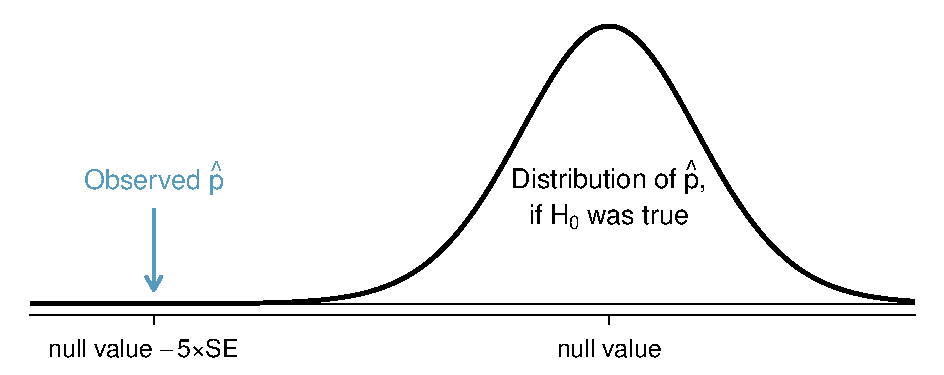
\includegraphics[width=0.75\textwidth]{ch_inference_for_props/figures/whyWeWantPValue/whyWeWantPValueProp}
\caption{It would be helpful to quantify the strength of the evidence against the null hypothesis. In this case, the evidence is extremely strong.}
\label{whyWeWantPValue}
\end{figure}



\subsection{Formal testing using p-values}

\label{pValue}

\index{hypothesis testing!p-value|(}

The p-value is a way of quantifying the strength of the evidence against the null hypothesis and in favor of the alternative. Formally the \emph{p-value} is a conditional probability.

\begin{termBox}{\tBoxTitle{p-value}
The \term{p-value}\index{hypothesis testing!p-value|textbf} is the probability of observing data at least as favorable to the alternative hypothesis as our current data set, if the null hypothesis is true. We typically use a summary statistic of the data, in this section the sample proportion, to help compute the p-value and evaluate the hypotheses.}
\end{termBox}

Statistical hypothesis testing almost always uses the p-value method rather than confidence intervals. In this formal space of hypothesis testing for proportions, we will slightly modify how we check the success-failure condition and compute the standard error. These changes aren't dramatic, but they will require paying a little more attention to how we use the null value, $p_0$.

%To apply the normal distribution framework in the context of a hypothesis test for a proportion, the independence and success-failure conditions must be satisfied. In a hypothesis test, the success-failure condition is checked using the null proportion: we verify $np_0$ and $n(1-p_0)$ are at least 10, where $p_0$ is the null value.

\index{data!coal power support|(}

\begin{example}{Pew Research asked a random sample of 1000 American
    adults whether they supported the increased usage of
    coal. Set up hypotheses to evaluate whether this represents
    a majority of Americans, one way or the other.}
  The uninteresting result is that there is no majority either way:
  half of Americans support and the other half oppose expanding the
  use of coal to produce energy. The alternative hypothesis would
  be that there is a majority support (or oppose) to expanding the
  use of coal. If $p$ represents the proportion supporting, then
  we can write the hypotheses as
  \begin{description}
    \item[$H_0$:] $p = 0.5$
    \item[$H_A$:] $p \neq 0.5$
  \end{description}
  In this case, the null value ($p_0$) is 0.5.
\end{example}

Pew Research's sample found that 37\% of American adults support
increased usage of coal. We now wonder, does 37\% represent a
real difference from the null hypothesis of 50\%.

\begin{example}{What would the sampling distribution of $\hat{p}$
    look like if the null hypothesis were true?}
  If the null hypothesis were true, the population proportion
  would be the null value, 0.5. We previously learned that
  the sampling distribution of $\hat{p}$ will be normal when
  two conditions are met:
  \begin{itemize}
    \item Independence is reasonable since this poll is based on
        a simple random sample.
    \item Based on the poll's sample size of $n = 1000$,
        the success-failure condition is met, since
        \begin{align*}
        np \quad \stackrel{H_0}{=} \quad 1000 \times 0.5 = 500
        \qquad
        n (1 - p) \quad \stackrel{H_0}{=} \quad 1000 \times (1 - 0.5) = 500
        \end{align*}
        are both greater than 10. Note that the success-failure
        condition was checked using the null value, $p_0 = 0.5$;
        this is the first procedural difference from confidence
        intervals.
  \end{itemize}
  If the null hypothesis were true, the sampling distribution
  indicates that a sample proportion based on $n = 1000$ observations
  would be normally distributed. Next, we can compute the standard
  error, where we will again use the null value $p_0 = 0.5$ in the
  calculation:
  \begin{align*}
  SE = \sqrt{\frac{p (1 - p)}{n}}
      \quad \stackrel{H_0}{=} \quad \sqrt{\frac{0.5 \times 0.5}{1000}}
      = 0.016
  \end{align*}
  This marks the other procedural difference from confidence
  intervals: since the sampling distribution is determined
  under the null proportion, the null value $p_0$ was used for
  the proportion in the calculation rather than $\hat{p}$.

  Ultimately, if the null hypothesis were true, then the sample
  proportion should follow a normal distribution with mean 0.500
  and standard error of 0.016. This distribution is shown in
  Figure~\ref{}. \Comment{Create this figure.}
\end{example}

When we identify the sampling distribution under the null hypothesis,
it has a special name: the \term{null distribution}. The p-value
represents the probability of the observed $\hat{p}$, or a $\hat{p}$
that is more extreme, if the null hypothesis were true.

\begin{example}{Compute the chance that $\hat{p} = 0.36$ or
    further from 0.5 under the null distribution, which is a
    normal distribution with mean 0.5 and $SE = 0.016$.}
  This is a normal probability problem where $x = 0.36$.
  First, we draw a simple graph to represent the situation,
  similar to what is shown in Figure~\ref{}.
  \Comment{Add figure ref.}
  Since $\hat{p}$ is so far out in the tail, we know the
  tail area is going to be very small. To find it, we start
  by computing the Z-score using the mean of 0.5 and the
  standard error of 0.016:
  \begin{align*}
  Z = \frac{0.37 - 0.5}{0.016} = 8.125 
  \end{align*}
  We can use the normal probability table or software to find
  the tail area. If we use the probability table, we consider the
  smallest Z-score shown, which in Appendix~\ref{} corresponds
  to a tail area of 0.0002.

  To get the p-value, we double this tail area, since observations
  in the mirror-imaged tail (Figure~\ref{}) are also just as extreme
  relative to 0.5 as those below 0.37.
  \Comment{Create this new figure.}
  This gives a p-value of 0.0004.

  Here, the p-value represents the probability of observing
  such an extreme sample proportion by chance, if the null hypothesis
  were true.
\end{example}

\begin{example}{How should we evaluate the hypotheses using the
    p-value of 0.0004? Use the standard significance level of
    $\alpha = 0.05$.}
  If the null hypothesis were true, it's very unlikely that we would
  observe such an extreme deviation of $\hat{p}$ from 0.5. This means
  there are one of two possibilities:
  \begin{enumerate}
    \item The null hypothesis is true, and we just happened to get
        really unlucky.
    \item The alternative hypothesis is true, which would be consistent
        with observing a sample proportion far from 0.5.
  \end{enumerate}
  The p-value tells us that what we observed is so unusual
  with respect to null hypothesis that it casts serious doubt on $H_0$.
  Formally, we compare the p-value to the significance level
  $\alpha = 0.05$. Since the p-value is less than $\alpha$,
  we reject the null hypothesis.
  That is, the data provide strong evidence against $H_0$,
  and we conclude that a majority of Americans do not support
  expanding the use of coal.
\end{example}

\index{data!coal power support|)}

\begin{tipBox}{
  \tipBoxTitle{Compare the p-value to $\mathbf{\alpha}$ to
      evaluate $\mathbf{H_0}$}
  When the p-value is less than the significance level, $\alpha$,
  reject $H_0$. We would report a conclusion that the data provide
  strong evidence supporting the alternative hypothesis. \\[2mm]
  When the p-value is greater than $\alpha$, do not reject $H_0$,
  and report that we do not have sufficient evidence to reject the
  null hypothesis. \\[2mm]
  In either case, it is important to describe the conclusion
  in the context of the data.}
\end{tipBox}







\index{data!nuclear arms reduction|(}

\begin{exercise}
Do a majority of American support or oppose nuclear arms reduction? Set up hypotheses to evaluate this question.\footnote{We would like to understand if a majority supports or opposes, or ultimately, if there is no difference. $H_0: p = 0.50$. $H_A: p > 0.50$.}
\end{exercise}

\begin{example}{A simple random sample of 1,028 US adults in March 2013 found that 56\% support nuclear arms reduction.\footnote{\oiRedirect{textbook-nuclear_arms_reduction_201303}{www.gallup.com/poll/161198/favor-russian-nuclear-arms-reductions.aspx}} Does this provide convincing evidence that a majority of Americans supported nuclear arms reduction at the 5\% significance level?} \label{NuclearArmsInferenceExample}
The poll was of a simple random sample that includes fewer than 10\% of US adults, meaning the observations are independent. In a one-proportion hypothesis test, the success-failure condition is checked using the null proportion, which is $p_0 = 0.5$ in this context: $n p_0 = n (1 - p_0) = 1028 \times 0.5 = 514 > 10$. With these conditions verified, the normal model may be applied to $\hat{p}$.

Next the standard error can be computed. The null value $p_0$ is used again here, because this is a hypothesis test for a single proportion.
\begin{align*}
SE = \sqrt{\frac{p_0 (1 - p_0)}{n}} = \sqrt{\frac{0.5 (1 - 0.5)}{1028}} = 0.016
\end{align*}
A picture of the normal model is shown in Figure~\ref{nuclearArmsReductionPValue} with the p-value represented by the shaded region. Based on the normal model, the test statistic can be computed as the Z-score of the point estimate:
\begin{align*}
Z = \frac{\text{point estimate} - \text{null value}}{SE} = \frac{0.56 - 0.50}{0.016} = 3.75
\end{align*}
The upper tail area, representing the p-value, is about 0.0001. Because the p-value is smaller than 0.05, we reject $H_0$. The poll provides convincing evidence that a majority of Americans supported nuclear arms reduction efforts in March 2013.
\end{example}

\begin{figure}[h]
\centering
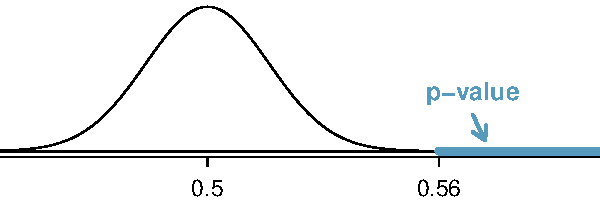
\includegraphics[width=0.48\textwidth]{ch_inference_for_props/figures/nuclearArmsReduction/nuclearArmsReductionPValue}
\caption{Sampling distribution for Example~\ref{NuclearArmsInferenceExample}.}
\label{nuclearArmsReductionPValue}
\end{figure}

\begin{termBox}{\tBoxTitle{Hypothesis test for a proportion}
Set up hypotheses and verify the conditions using the null value, $p_0$, to ensure $\hat{p}$ is nearly normal under $H_0$. If the conditions hold, construct the standard error, again using $p_0$, and show the p-value in a drawing. Lastly, compute the p-value and evaluate the hypotheses.}
\end{termBox}

\index{data!nuclear arms reduction|)}

\begin{tipBox}{\tipBoxTitle{One-sided and two-sided tests}
When you are interested in checking for an increase or a decrease, but not both, use a one-sided test. When you are interested in any difference from the null value~--~an increase or decrease~--~then the test should be two-sided.\vspace{0.5mm}}
\end{tipBox}

\begin{tipBox}{\tipBoxTitle{Always write the null hypothesis as an equality}
We will find it most useful if we always list the null hypothesis as an equality (e.g. $\mu = 7$) while the alternative always uses an inequality (e.g. $\mu\neq7$, $\mu>7$, or $\mu<7$).}
\end{tipBox}

The researchers at the rural school conducted a simple random sample of $n=110$ students on campus. They found that these students averaged 7.42 hours of sleep and the standard deviation of the amount of sleep for the students was 1.75 hours. A histogram of the sample is shown in Figure~\ref{histOfSleepForCollegeThatWasCheckingForMoreThan7Hours}.

\begin{figure}
\centering
%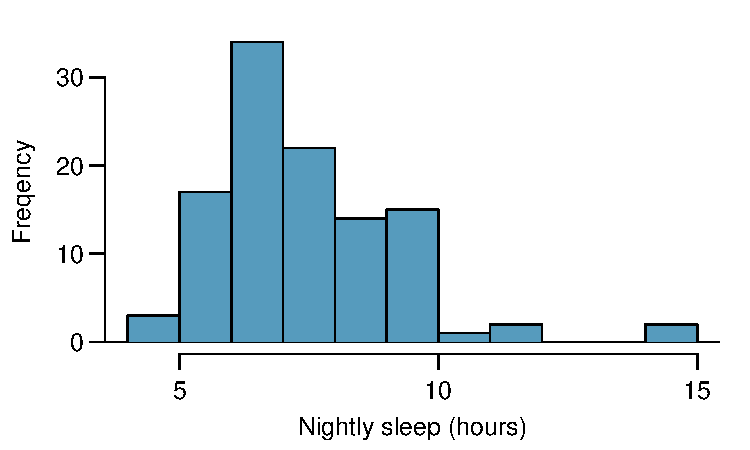
\includegraphics[width=0.7\textwidth]{ch_inference_foundations/figures/histOfSleepForCollegeThatWasCheckingForMoreThan7Hours/histOfSleepForCollegeThatWasCheckingForMoreThan7Hours}
\caption{Distribution of a night of sleep for 110 college students. These data are strongly skewed.\index{skew!example: strong}}
\label{histOfSleepForCollegeThatWasCheckingForMoreThan7Hours}
\end{figure}

Before we can use a normal model for the sample mean or compute the standard error of the sample mean, we must verify conditions. (1)~Because this is a simple random sample from less than 10\% of the student body, the observations are independent. (2)~The sample size in the sleep study is sufficiently large since it is greater than 30. (3)~The data show strong skew in Figure~\ref{histOfSleepForCollegeThatWasCheckingForMoreThan7Hours} and the presence of a couple of outliers. This skew and the outliers are acceptable for a sample size of $n=110$. With these conditions verified, the normal model can be safely applied to $\bar{x}$ and we can reasonably calculate the standard error.

\begin{exercise} \label{findSEOfFirstSleepStudyCheckingGreaterThan7Hours}
In the sleep study, the sample standard deviation was 1.75 hours and the sample size is 110. Calculate the standard error of $\bar{x}$.\footnote{The standard error can be estimated from the sample standard deviation and the sample size: $SE_{\bar{x}} = \frac{s_x}{\sqrt{n}} = \frac{1.75}{\sqrt{110}} = 0.17$.}
\end{exercise}

The hypothesis test for the sleep study will be evaluated using a significance level of $\alpha = 0.05$. We want to consider the data under the scenario that the null hypothesis is true. In this case, the sample mean is from a distribution that is nearly normal and has mean 7 and standard deviation of about $SE_{\bar{x}} = 0.17$. Such a distribution is shown in Figure~\ref{pValueOneSidedSleepStudy}.

\begin{figure}[hht]
   \centering
%   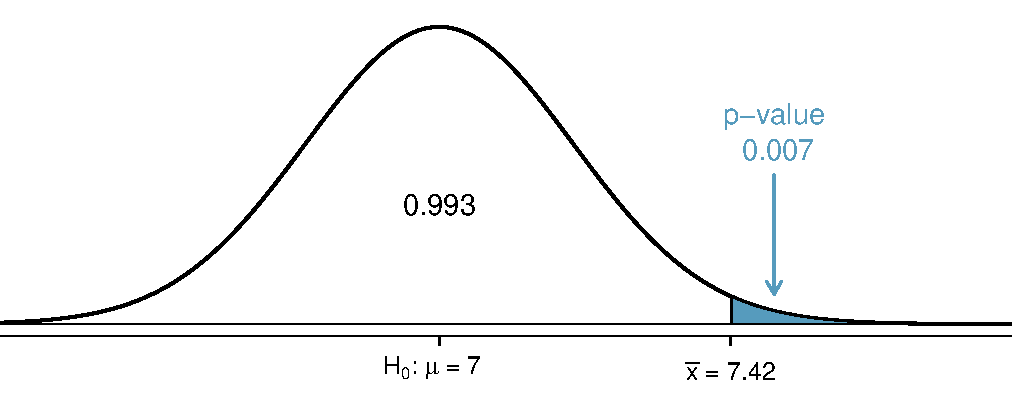
\includegraphics[width=0.83\textwidth]{ch_inference_foundations/figures/pValueOneSidedSleepStudy/pValueOneSidedSleepStudy}
   \caption{If the null hypothesis is true, then the sample mean $\bar{x}$ came from this nearly normal distribution. The right tail describes the probability of observing such a large sample mean if the null hypothesis is true.}
   \label{pValueOneSidedSleepStudy}
\end{figure}

The shaded tail in Figure~\ref{pValueOneSidedSleepStudy} represents the chance of observing such a large mean, conditional on the null hypothesis being true. That is, the shaded tail represents the \mbox{p-value}. We shade all means larger than our sample mean, $\bar{x} = 7.42$, because they are more favorable to the alternative hypothesis than the observed mean.

We compute the p-value by finding the tail area of this normal distribution, which we learned to do in Section~\ref{normalDist}. First compute the Z-score of the sample mean, $\bar{x} = 7.42$:
\begin{eqnarray*}
Z = \frac{\bar{x} - \text{null value}}{SE_{\bar{x}}} = \frac{7.42 - 7}{0.17} = 2.47
\end{eqnarray*}
Using the normal probability table, the lower unshaded area is found to be 0.993. Thus the shaded area is $1-0.993 = 0.007$. {\em If the null hypothesis is true, the probability of observing a sample mean at least as large as 7.42 hours for a sample of 110 students is only 0.007.}\index{p-value!interpretation example} That is, if the null hypothesis is true, we would not often see such a large mean.

We evaluate the hypotheses by comparing the p-value to the significance level. Because the p-value is less than the significance level (p-value $=0.007 < 0.05=\alpha$), we reject the null hypothesis. What we observed is so unusual with respect to the null hypothesis that it casts serious doubt on $H_0$ and provides strong evidence favoring $H_A$.

\begin{termBox}{\tBoxTitle{p-value as a tool in hypothesis testing}
The smaller the p-value, the stronger the data favor $H_A$ over $H_0$. A small p-value (usually $<0.05$) corresponds to sufficient evidence to reject $H_0$ in favor of $H_A$.}
\index{hypothesis testing!p-value|)}
\end{termBox}

\begin{tipBox}{\tipBoxTitle{It is useful to first draw a picture to find the p-value}
It is useful to draw a picture of the distribution of $\bar{x}$ as though $H_0$ was true (i.e.~$\mu$~equals the null value), and shade the region (or regions) of sample means that are at least as favorable to the alternative hypothesis. These shaded regions represent the p-value.}
\end{tipBox}

The ideas below review the process of evaluating hypothesis tests with p-values:
\begin{itemize}
\setlength{\itemsep}{0mm}
\item The null hypothesis represents a skeptic's position or a position of no difference. We reject this position only if the evidence strongly favors $H_A$.
\item A small p-value means that if the null hypothesis is true, there is a low probability of seeing a point estimate at least as extreme as the one we saw. We interpret this as strong evidence in favor of the alternative.
\item We reject the null hypothesis if the p-value is smaller than the significance level, $\alpha$, which is usually 0.05. Otherwise, we fail to reject $H_0$.
\item We should always state the conclusion of the hypothesis test in plain language so folks who aren't data scientists can also understand the results.
\end{itemize}

The p-value is constructed in such a way that we can directly compare it to the significance level ($\alpha$) to determine whether or not to reject $H_0$. This method ensures that the Type~1 Error rate does not exceed the significance level standard. 

\begin{figure}[ht]
   \centering
%   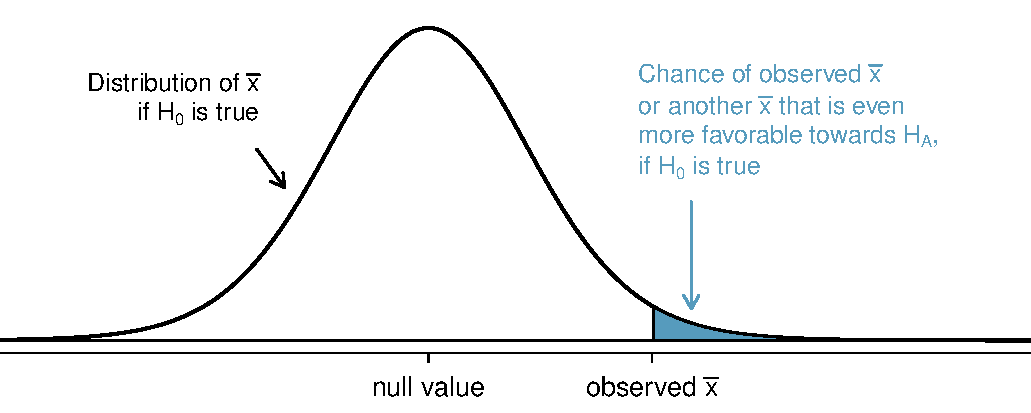
\includegraphics[width=0.9\textwidth]{ch_inference_foundations/figures/pValueOneSidedSleepStudyExplained/pValueOneSidedSleepStudyExplained}
   \caption{To identify the p-value, the distribution of the sample mean is considered as if the null hypothesis was true. Then the p-value is defined and computed as the probability of the observed $\bar{x}$ or an $\bar{x}$ even more favorable to $H_A$ under this distribution.}
   \label{pValueOneSidedSleepStudyExplained}
\end{figure}

\begin{exercise}
If the null hypothesis is true, how often should the p-value be less than 0.05?\footnote{About 5\% of the time. If the null hypothesis is true, then the data only has a 5\% chance of being in the 5\% of data most favorable to $H_A$.}
\index{data!school sleep|)}
\end{exercise}

\begin{exercise}
Suppose we had used a significance level of 0.01 in the sleep study. Would the evidence have been strong enough to reject the null hypothesis? (The p-value was 0.007.) What if the significance level was $\alpha = 0.001$? \footnote{We reject the null hypothesis whenever $p$-$value < \alpha$. Thus, we would still reject the null hypothesis if $\alpha = 0.01$ but not if the significance level had been $\alpha = 0.001$.}
\end{exercise}

\begin{exercise} \label{ebayAmazonOneSidedTestExercise}
\index{data!mario\_kart|(}
Ebay might be interested in showing that buyers on its site tend to pay less than they would for the corresponding new item on Amazon. We'll research this topic for one particular product: a video game called \emph{Mario Kart} for the Nintendo Wii. During early October 2009, Amazon sold this game for \$46.99. Set up an appropriate (one-sided!) hypothesis test to check the claim that Ebay buyers pay less during auctions at this same time.\footnote{The skeptic would say the average is the same on Ebay, and we are interested in showing the average price is lower.
\begin{itemize}
\setlength{\itemsep}{0mm}
\item[$H_0$:] The average auction price on Ebay is equal to (or more than) the price on Amazon. We write only the equality in the statistical notation: $\mu_{ebay} = 46.99$.
\item[$H_A$:] The average price on Ebay is less than the price on Amazon, $\mu_{ebay} < 46.99$.
\end{itemize}}
\end{exercise}


\begin{exercise} \label
{exerciseFor52EbayAuctionsToExamineMarioKartLessExpensiveThanAmazonConditions}
During early October 2009, 52 Ebay auctions were recorded for \emph{Mario Kart}.\footnote{These data were collected by OpenIntro staff.} The total prices for the auctions are presented using a histogram in Figure~\ref{ebayMarioKartAuctionPriceHistogramFor3ConditionsExercise}, and we may like to apply the normal model to the sample mean. Check the three conditions required for applying the normal model: (1)~independence, (2)~at~least 30 observations, and (3)~the data are not strongly skewed.\footnote{(1) The independence condition is unclear. \emph{We will make the assumption that the observations are independent, which we should report with any final results.} (2) The sample size is sufficiently large: $n =52 \geq 30$. (3) The data distribution is not strongly skewed; it is approximately symmetric.}
\end{exercise}

\begin{figure}
   \centering
%   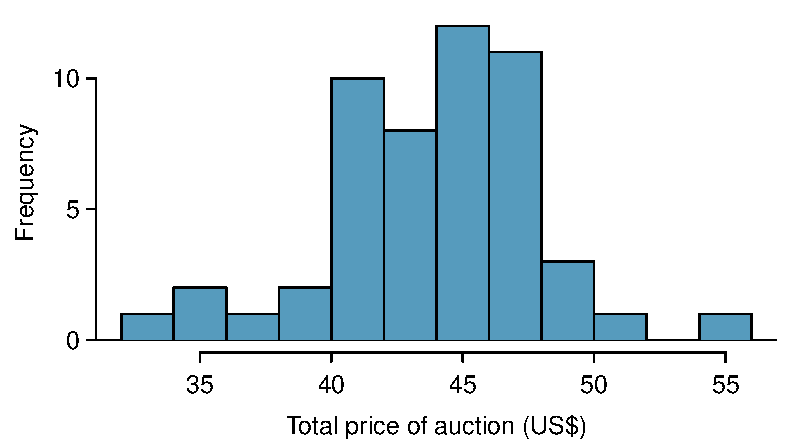
\includegraphics[width=0.77\textwidth]{ch_inference_foundations/figures/ebayMarioKartAuctionPriceHistogramFor3ConditionsExercise/ebayMarioKartAuctionPriceHistogramFor3ConditionsExercise}
   \caption{A histogram of the total auction prices for 52 Ebay auctions.}
   \label{ebayMarioKartAuctionPriceHistogramFor3ConditionsExercise}
\end{figure}

\begin{example}{The average sale price of the 52 Ebay auctions for \emph{Wii Mario Kart} was \$44.17 with a standard deviation of \$4.15. Does this provide sufficient evidence to reject the null hypothesis in Guided Practice~\ref{ebayAmazonOneSidedTestExercise}? Use a significance level of $\alpha = 0.01$.}
The hypotheses were set up and the conditions were checked in Exercises~\ref{ebayAmazonOneSidedTestExercise} and~\ref{exerciseFor52EbayAuctionsToExamineMarioKartLessExpensiveThanAmazonConditions}. The next step is to find the standard error of the sample mean and produce a sketch to help find the p-value.
\begin{eqnarray*}
SE_{\bar{x}} = s/\sqrt{n} = 4.15/\sqrt{52} = 0.5755
\end{eqnarray*}
\begin{center}
%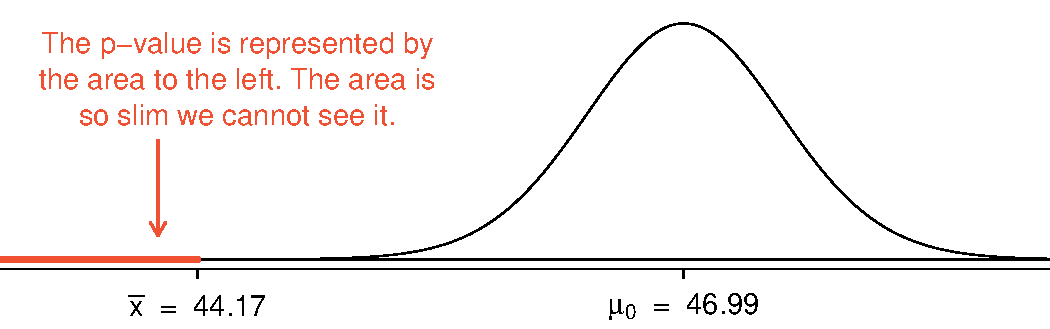
\includegraphics[height=35mm]{ch_inference_foundations/figures/pVForEbayAmazonComparison/pVForEbayAmazonComparison}
\end{center}
Because the alternative hypothesis says we are looking for a smaller mean, we shade the lower tail. We find this shaded area by using the Z-score and normal probability table: $Z = \frac{44.17 - 46.99}{0.5755} = -4.90$, which has area less than 0.0002. The area is so small we cannot really see it on the picture. This lower tail area corresponds to the p-value.

Because the p-value is so small -- specifically, smaller than $\alpha = 0.01$ -- this provides sufficiently strong evidence to reject the null hypothesis in favor of the alternative. The data provide statistically significant evidence that the average price on Ebay is lower than Amazon's asking price.
\index{data!mario\_kart|)}
\end{example}

\begin{termBox}{\tBoxTitle{What's so special about 0.05?}
It's common to use a threshold of 0.05 to determine whether a result is statistically significant, but why is the most common value 0.05? Maybe the standard significance level should be bigger, or maybe it should be smaller. If you're a little puzzled, that probably means you're reading with a critical eye -- good job! We've made a 5-minute task to help clarify \emph{why 0.05}:
\begin{center}
\oiRedirect{textbook-why05}{www.openintro.org/why05}
\end{center}
Sometimes it's also a good idea to deviate from the standard. We'll discuss when to choose a threshold different than 0.05 in Section~\ref{significanceLevel}.\vspace{0.5mm}}
\end{termBox}


\subsection{Two-sided hypothesis testing with p-values}
\label{twoSidedTestsWithPValues}






\CalculatorVideos{hypothesis tests for a single proportion}

\index{hypothesis testing|)}















\section{Better understanding the Central Limit Theorem}


\subsection{Why do we have the $np \geq 10$ and
    $n(1-p) \geq 10$ rules?}

We've only looked at one situation so far: when the sample
proportion is $p = 0.56$ and the sample size is $n = 1000$.
What happens if we have a different proportion or sample size?

Let's start by considering different sample sizes.
Figure~\ref{sampling_X_prop_56p} shows the distribution of sample
proportions when the sample size is 5, 25, and 100. There are
two key takeaways:
\begin{itemize}
\item When the sample size is very small, the distribution has
very discrete properties: it doesn't look very smooth. However,
for larger sample sizes, the distribution looks smoother and
more like a normal distribution.
\item The bigger the sample size, the more often the estimate is
close to the population proportion $p = 0.56$. This is intuitive:
bigger samples will tend to produce more accurate estimates.
\end{itemize}

\begin{figure}
   \centering
   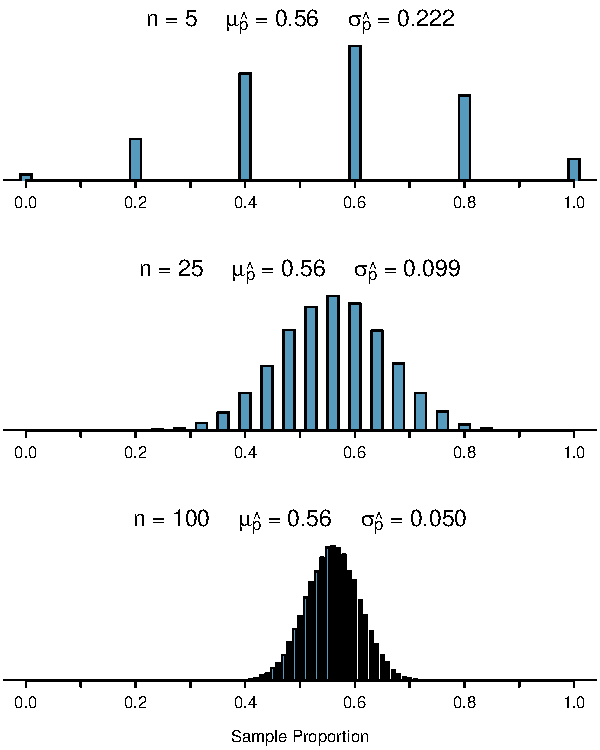
\includegraphics[width=0.67\textwidth]{ch_inference_for_props/figures/sampling_X_prop_56p/sampling_X_prop_56p}
   \caption{Simulations of $\hat{p}$ when the population
       proportion is $p = 0.56$ and for the following sample sizes:
       $n = 5$, $n = 25$, and $n = 100$. The theoretical
       mean~($\mu_{\hat{p}}$) and standard
       deviation~($SE_{\hat{p}}$) is also provided for each plot.}
   \label{sampling_X_prop_56p}
\end{figure}

%\begin{termBox}{\tBoxTitle{Law of Large Numbers for proportions}
%  \hiddenterm{Law of Large Numbers!proportions}
%  When the sample size is large, the sample proportion tends to be
%  a more reliable estimate of the population proportion.}
%\end{termBox}

Next let's consider what happens when we use different proportions.
For this exploration, let's use a sample size of $n = 100$ and
proportions of 0.03, 0.20, 0.50 0.80, and 0.97. The distributions
are shown in Figure~\ref{sampling_X_prop_56p}. Below are key
takeaways from these simulations:
\begin{itemize}
\item When the population proportion $p$ is close to 0 or 1, the
    distribution of sample proportions tends to be skewed. However,
    for proportions relatively far from   gets larger, the
    distribution becomes more symmetric
\item The estimates tend to be less variable when the proportion
    is near 0 or 1, as is shown by their lower variability listed
    in the table.
\end{itemize}

\begin{figure}
   \centering
   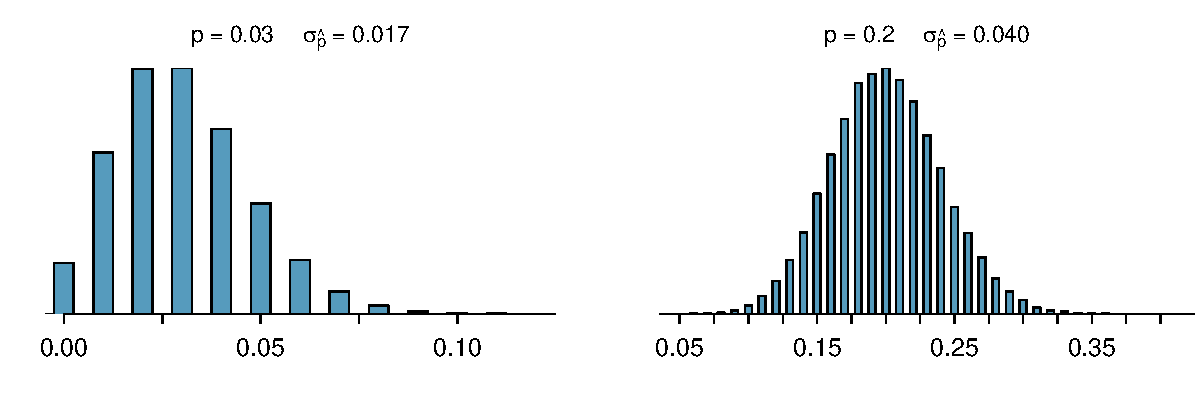
\includegraphics[width=\textwidth]{ch_inference_for_props/figures/sampling_100_prop_X/sampling_100_prop_X_12}
   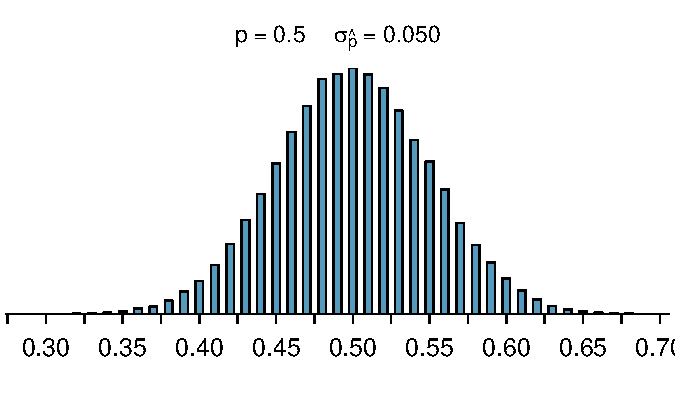
\includegraphics[width=0.55\textwidth]{ch_inference_for_props/figures/sampling_100_prop_X/sampling_100_prop_X_3}
   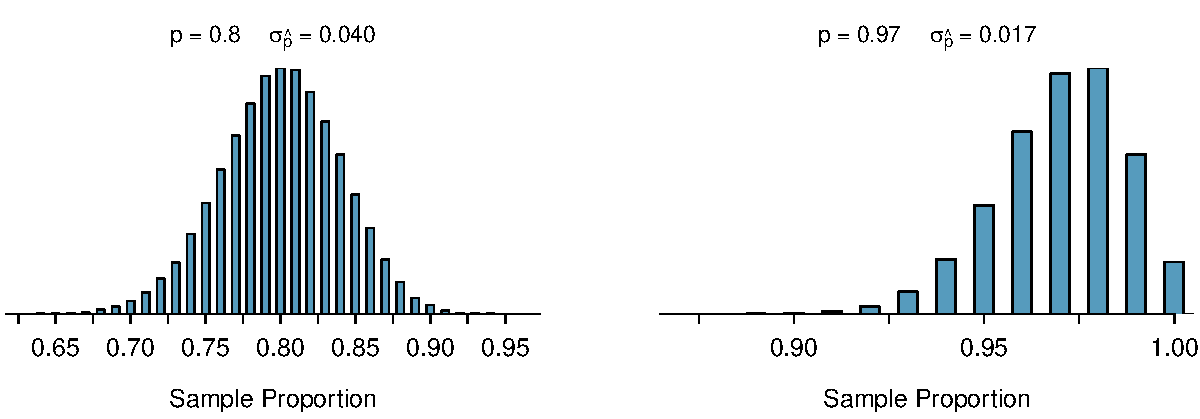
\includegraphics[width=\textwidth]{ch_inference_for_props/figures/sampling_100_prop_X/sampling_100_prop_X_45}
   \caption{Simulations of $\hat{p}$ for different population
       proportions when the sample size is $n = 100$. Each plot
       is centered at the population proportion $p$, and the
       theoretical standard deviation ($SE_{\hat{p}}$) is
       also provided for each plot.}
   \label{sampling_X_prop_56p}
\end{figure}

\Comment{Make sure the plots show $SE_{\hat{p}}$ rather than $\sigma_{\hat{p}}$.}


\subsection{Sampling distributions and the Central Limit Theorem}

In general, when we consider the distribution of a statistic, such as
a sample proportion, we call it a \term{sampling distribution}.
That is, the distribution shown in Figure~\ref{sampling_10k_prop_56p}
is a \emph{sampling distribution} for a sample proportion when the
sample size is 1000 and the population proportion is 0.56.

\begin{termBox}{\tBoxTitle{Sampling distribution}
  The sampling distribution represents the distribution of the point
  estimates based on samples of a fixed size from a certain population.
  It is useful to think of a particular point estimate as being drawn
  from such a distribution. Understanding the concept of a sampling
  distribution is central to understanding statistical inference.}
\end{termBox}

